\subsection{Prototyping}

Nachdem mithilfe der Nutzwertanalyse im Kapitel \ref{nutzwertanalyse} ein grundlegendes Gesamtkonzept festgelegt wurde, wird nun an Prototypen der einzelen Teilfunktionen gearbeitet. Das Ziel ist es, die einzelnen Teilfunktionen zu Testen und möglichst viele Fehler frühzeitig zu erkennen. Detaillierte Prototypen helfen die bereits bekannten Risiken besser einzuschätzen und neue Risiken frühzeitig zu erkennen.

\subsubsection{Greifer-Prototyp I}
\label{subsubsection:gripper-prototype-1}


Der Aufbau und die Funktionsweise des Greifers werden in Kapitel \ref{subsubsection:Hindernisse bewegen} erläutert. Um die Auslegung des Greifers \textbf{(REF AUSLEGUNG)} zu validieren und sein Funktionsprinzip zu überprüfen wurde ein Prototyp gebaut. Nachfolgend wurden die Ergebnisse aus den Tests am Protoyp dokumentiert

\textbf{Testaufbau}
 Der Prototyp besteht abgesehen von Befestigungselementen aus 3D-Druck Komponenten. der Aufbau wurde so gewählt, dass Iterationen an Einzelteilen schnell realisiert und verbaut werden können (Abb. \ref{fig:gripper-prototype-trimetric-notes}). 

\begin{figure}[H]
\centering
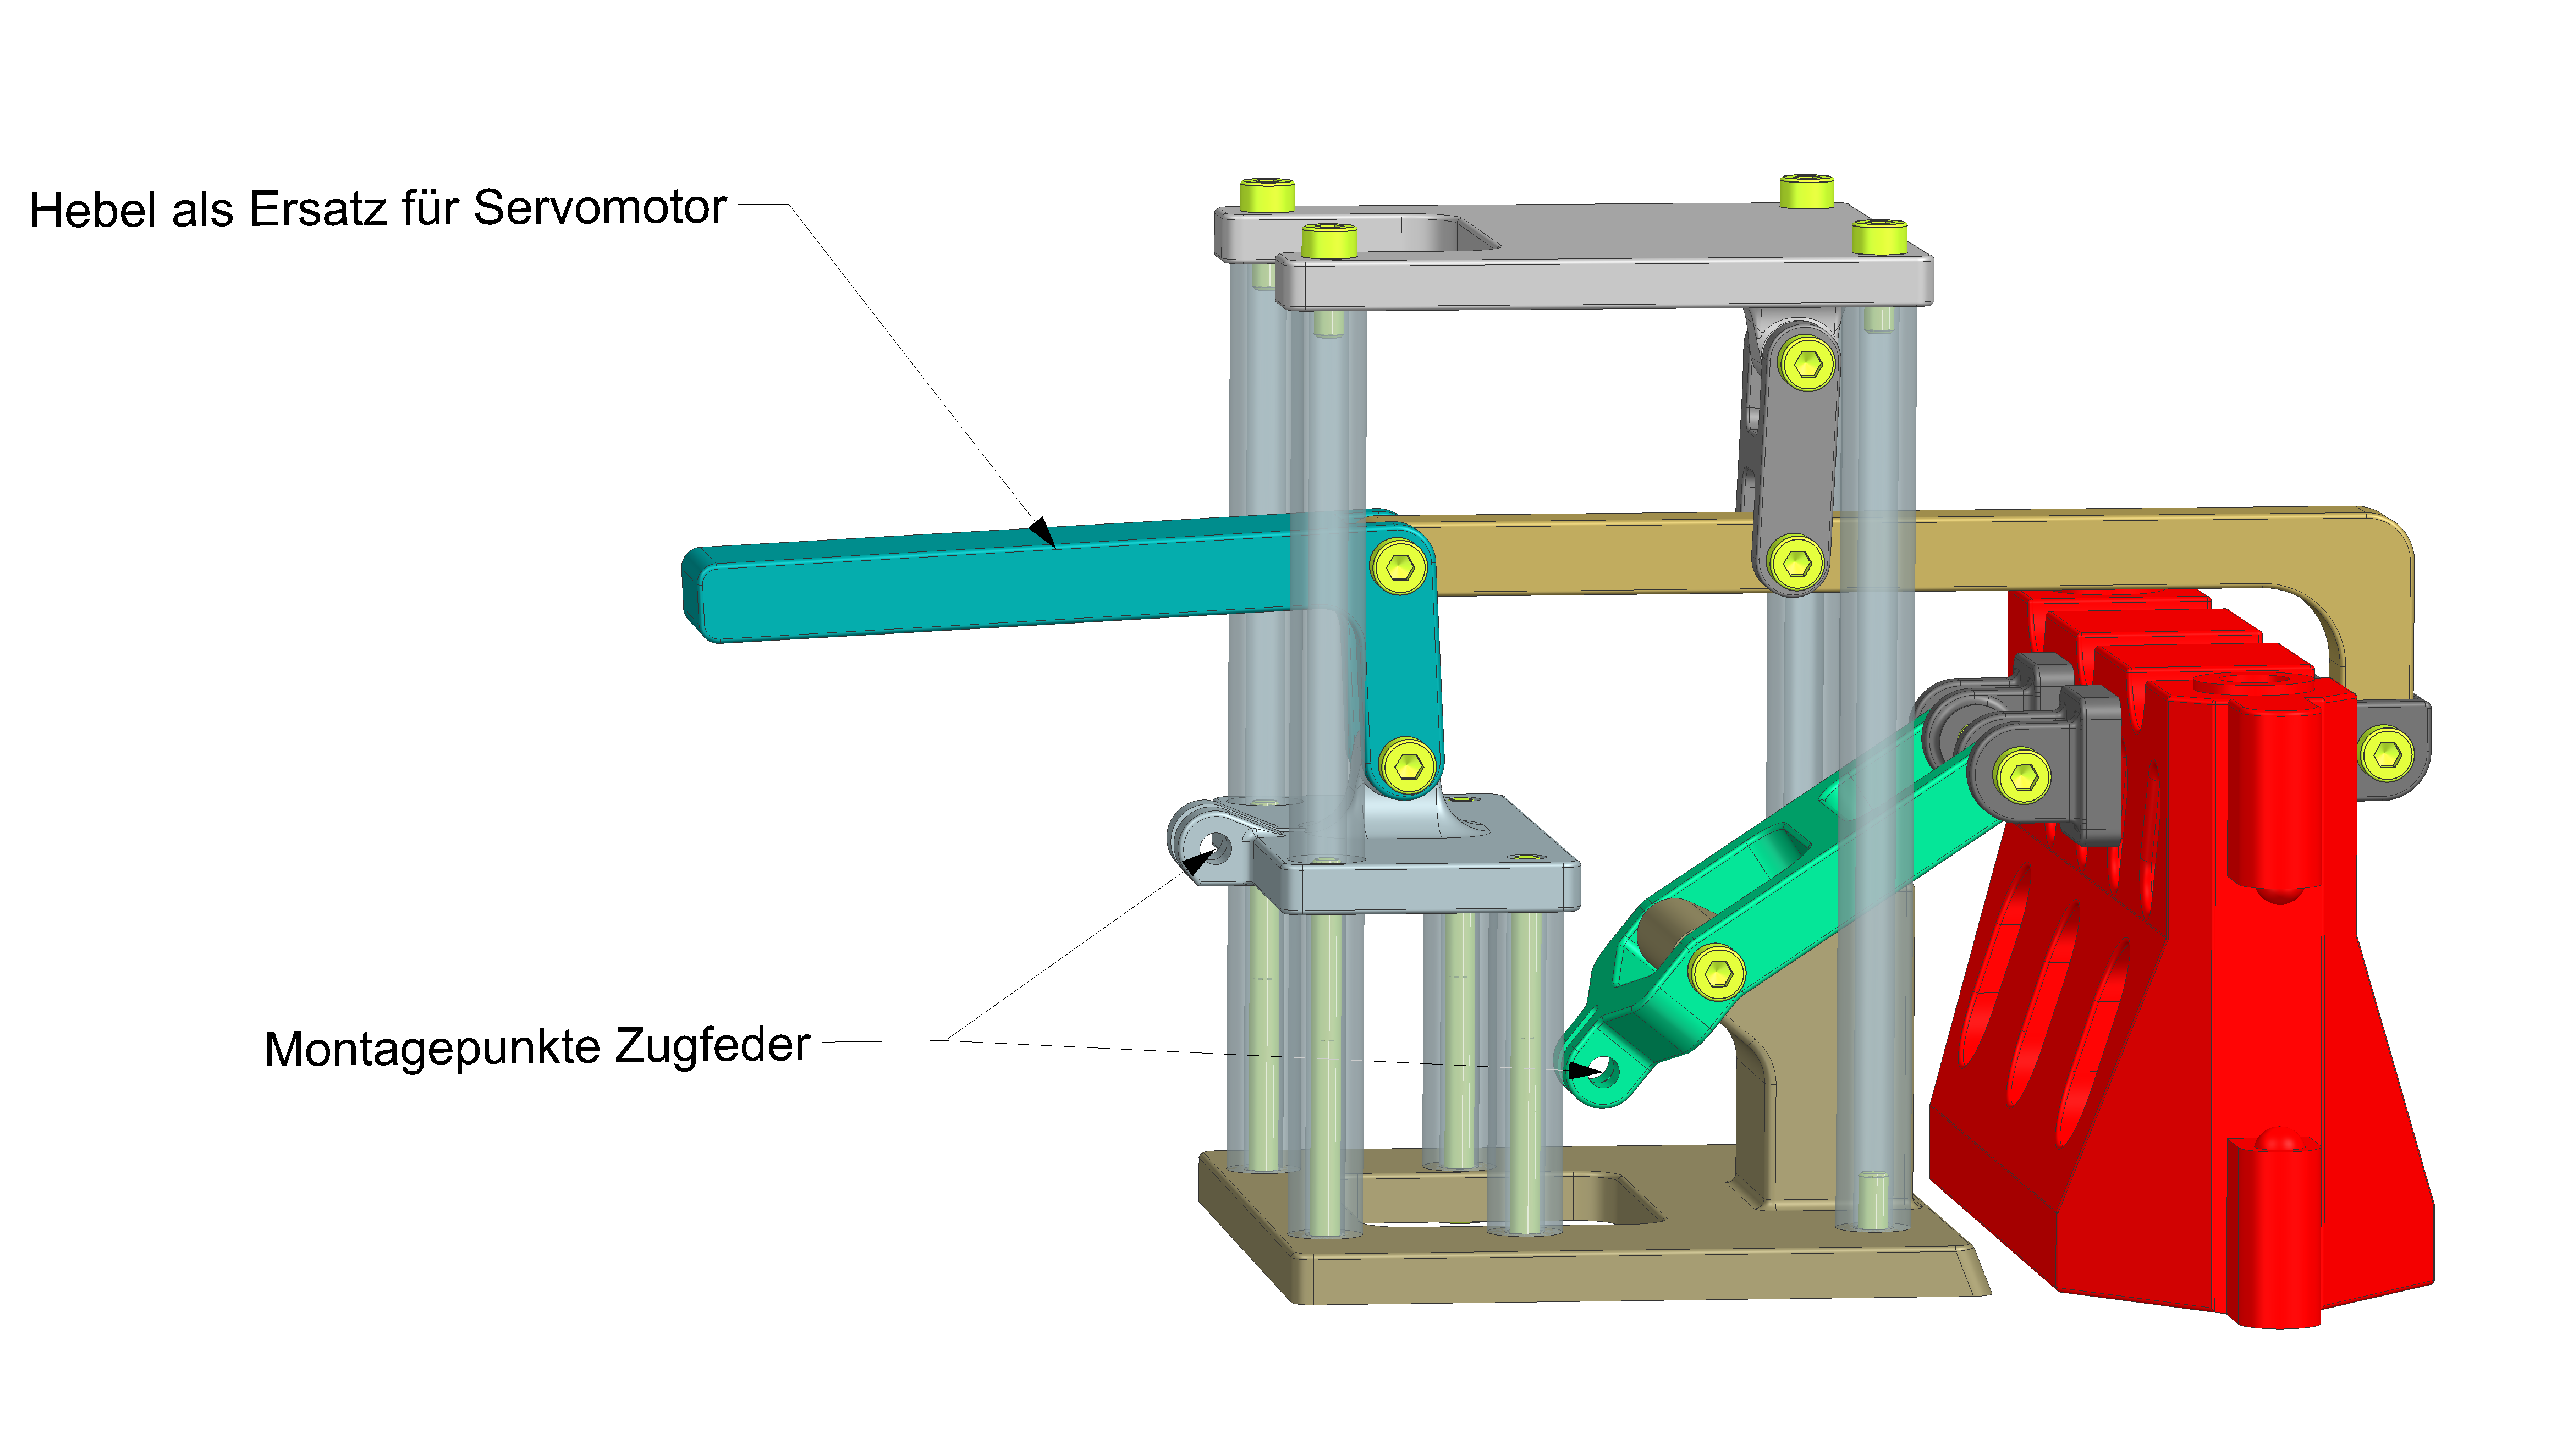
\includegraphics[width=1.0\textwidth]{assets/greifer-prototyp/Greifer_Trimetrisch_Notes.png}
\caption{Prototyp Greifer}
\label{fig:gripper-prototype-trimetric-notes}
\end{figure}

Der Prototyp wird manuell über einen Hebel bedient, welcher anstelle des Servomotors in der Konstruktion verbaut ist. Diese Entscheidung wurde getroffen, da das ausgelegte Motordrehmoment durch mögliche Reibung in den Gelenken nicht ausreichen könnte. Mit dem Hebel kann das ausgelegte Drehmoment einfach durch aufbringen einer bekannten Last validiert werden.
\\
Die Lagerpunkte des Gestänges wurden für den Prototyp an ein Gestell aufgebracht (Abb. \ref{fig:gripper-frame-mounting-points}). So kann der Greifer unabhängig vom Fahrzeug getestet werden. Die Abstände zwischen den Lagerpunkten sowie zum Boden sollen für den finalen Greifer dieselben sein. Auch die Dimensionen des Gestänges sollen beibehalten werden (Abb. \ref{fig:gripper-linkage-dimensions}). Somit bleiben die von der Geometrie abhängigen Kräfte dieselben und Ergebnisse aus Prototypentests können auf spätere Iterationen übertragen werden. 

\begin{figure}[H]
\begin{subfigure}{0.9\textwidth}
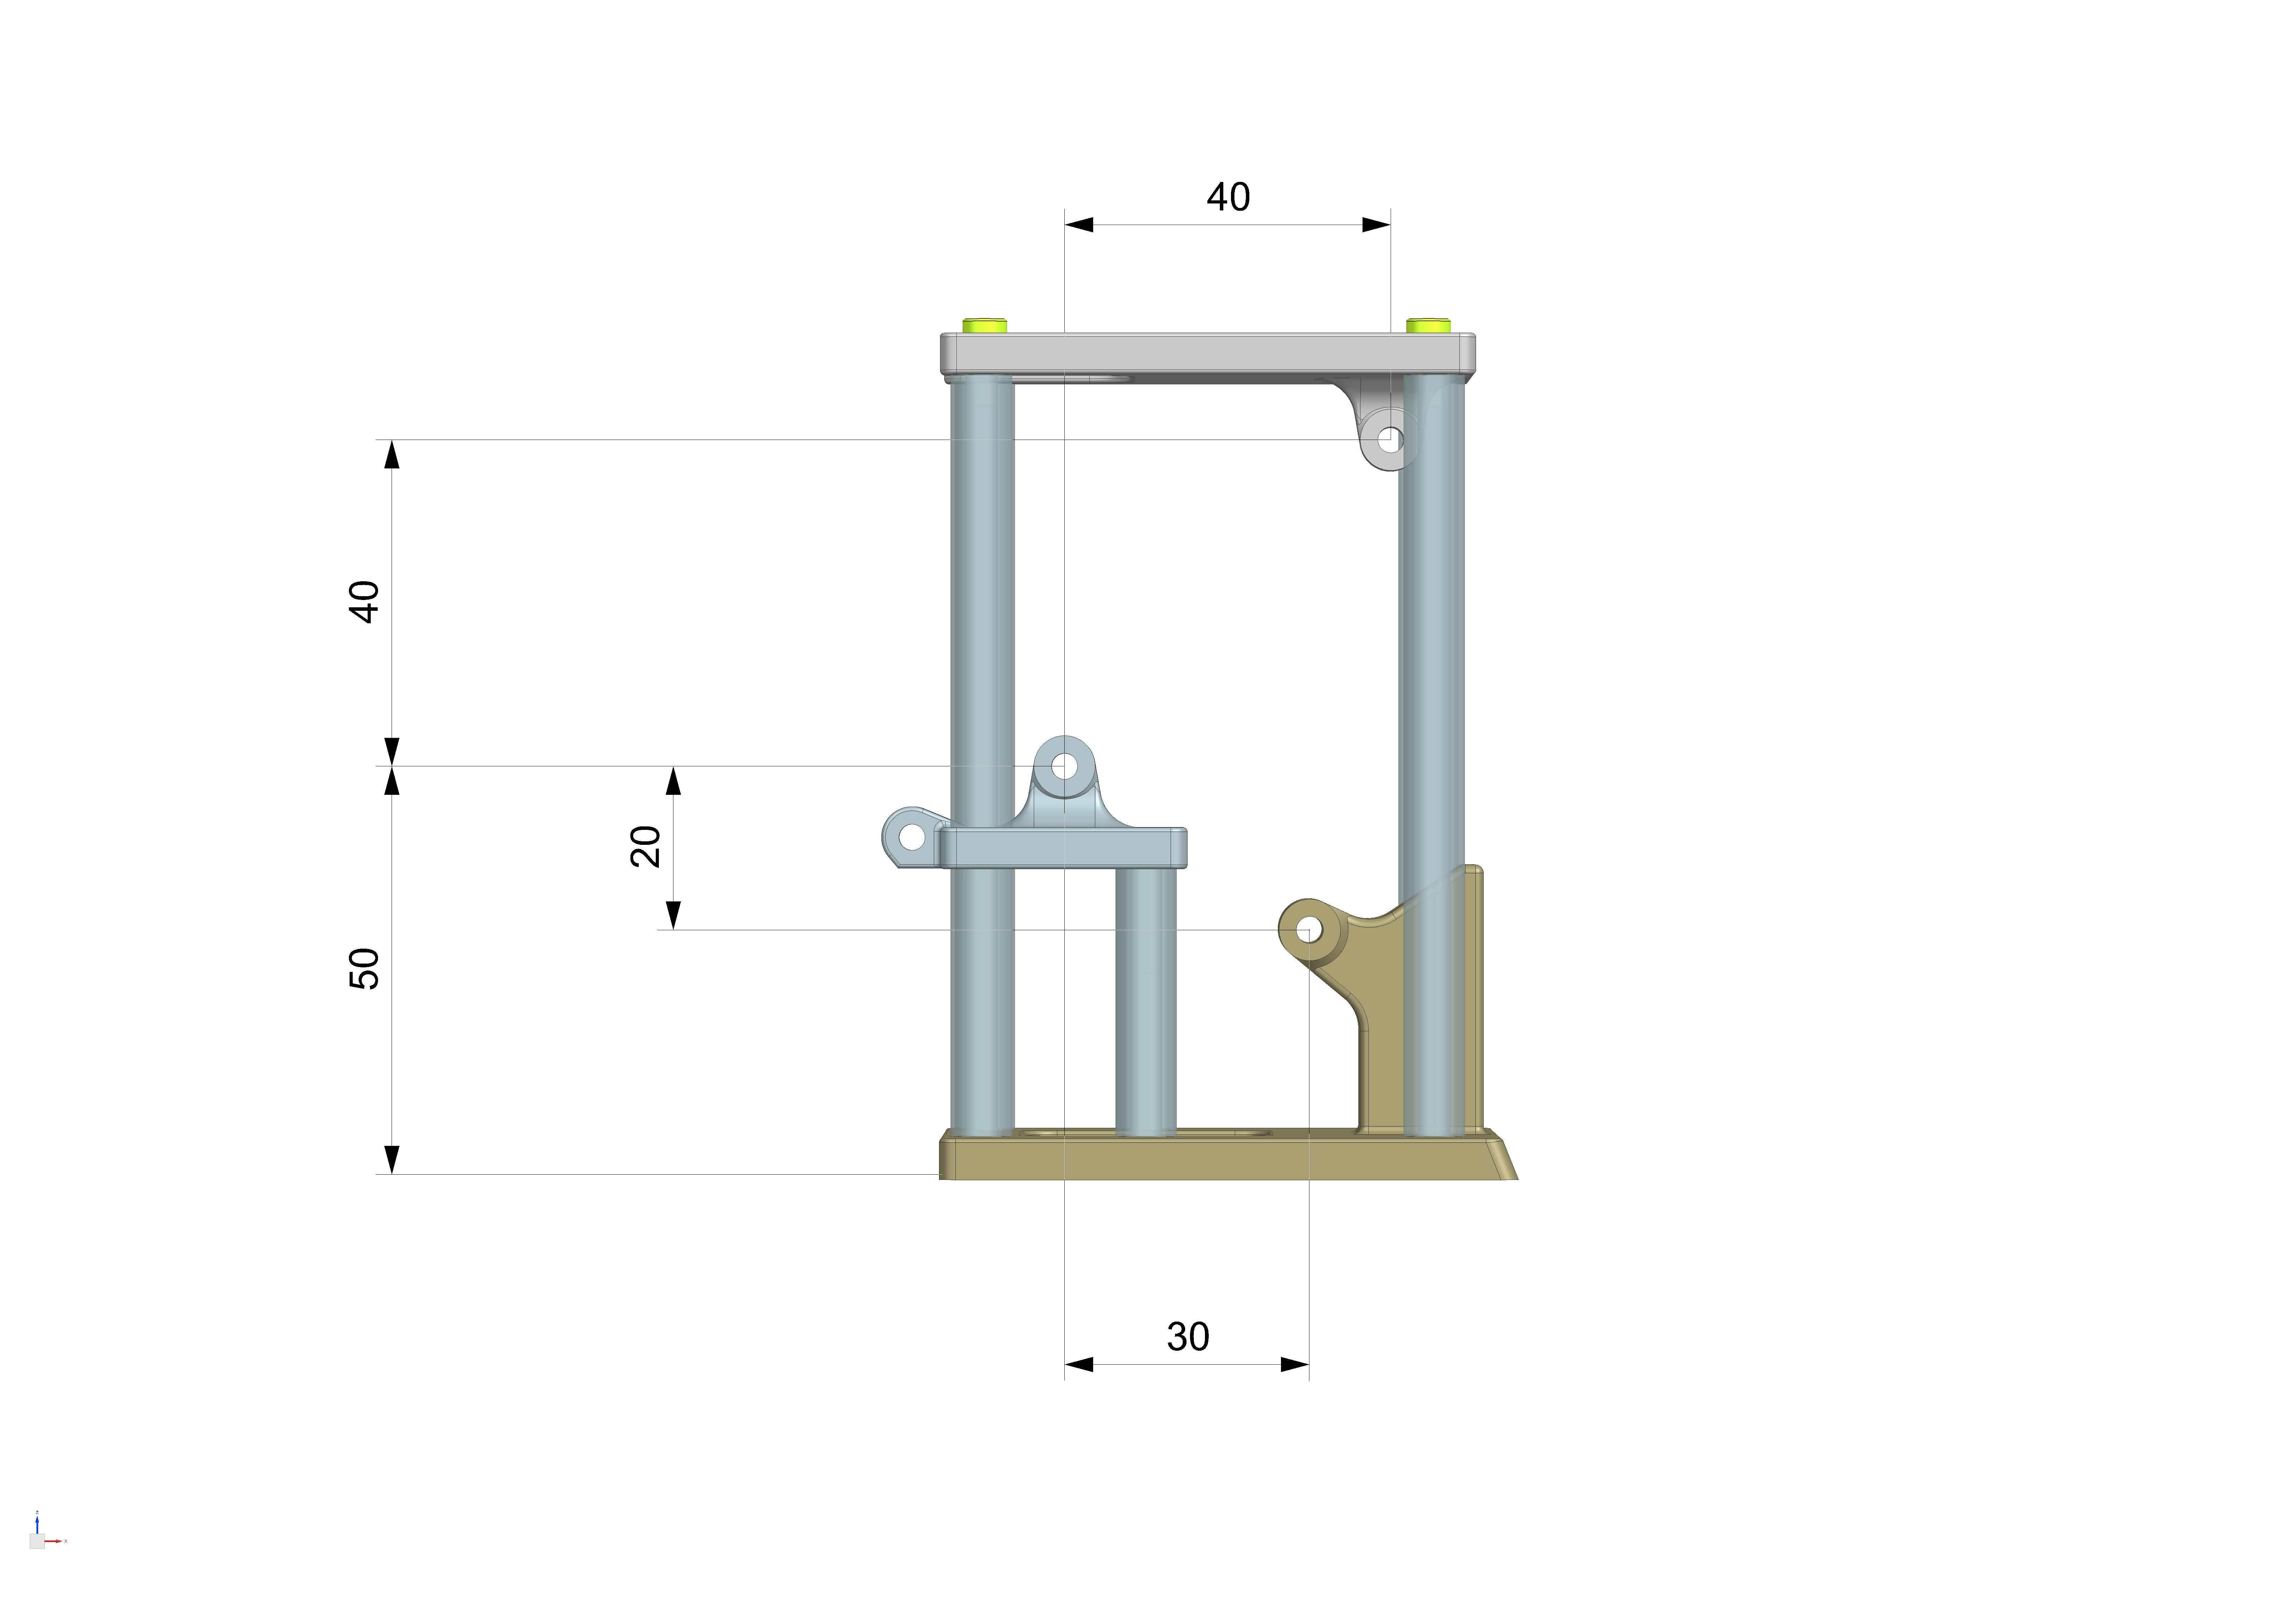
\includegraphics[width=\textwidth]{assets/greifer-prototyp/Greifer_Dimensionen_Lagerpunkte.png}
\caption{Gestell mit Lagerpunkten}
\label{fig:gripper-frame-mounting-points}
\end{subfigure}
\begin{subfigure}{0.9\textwidth}
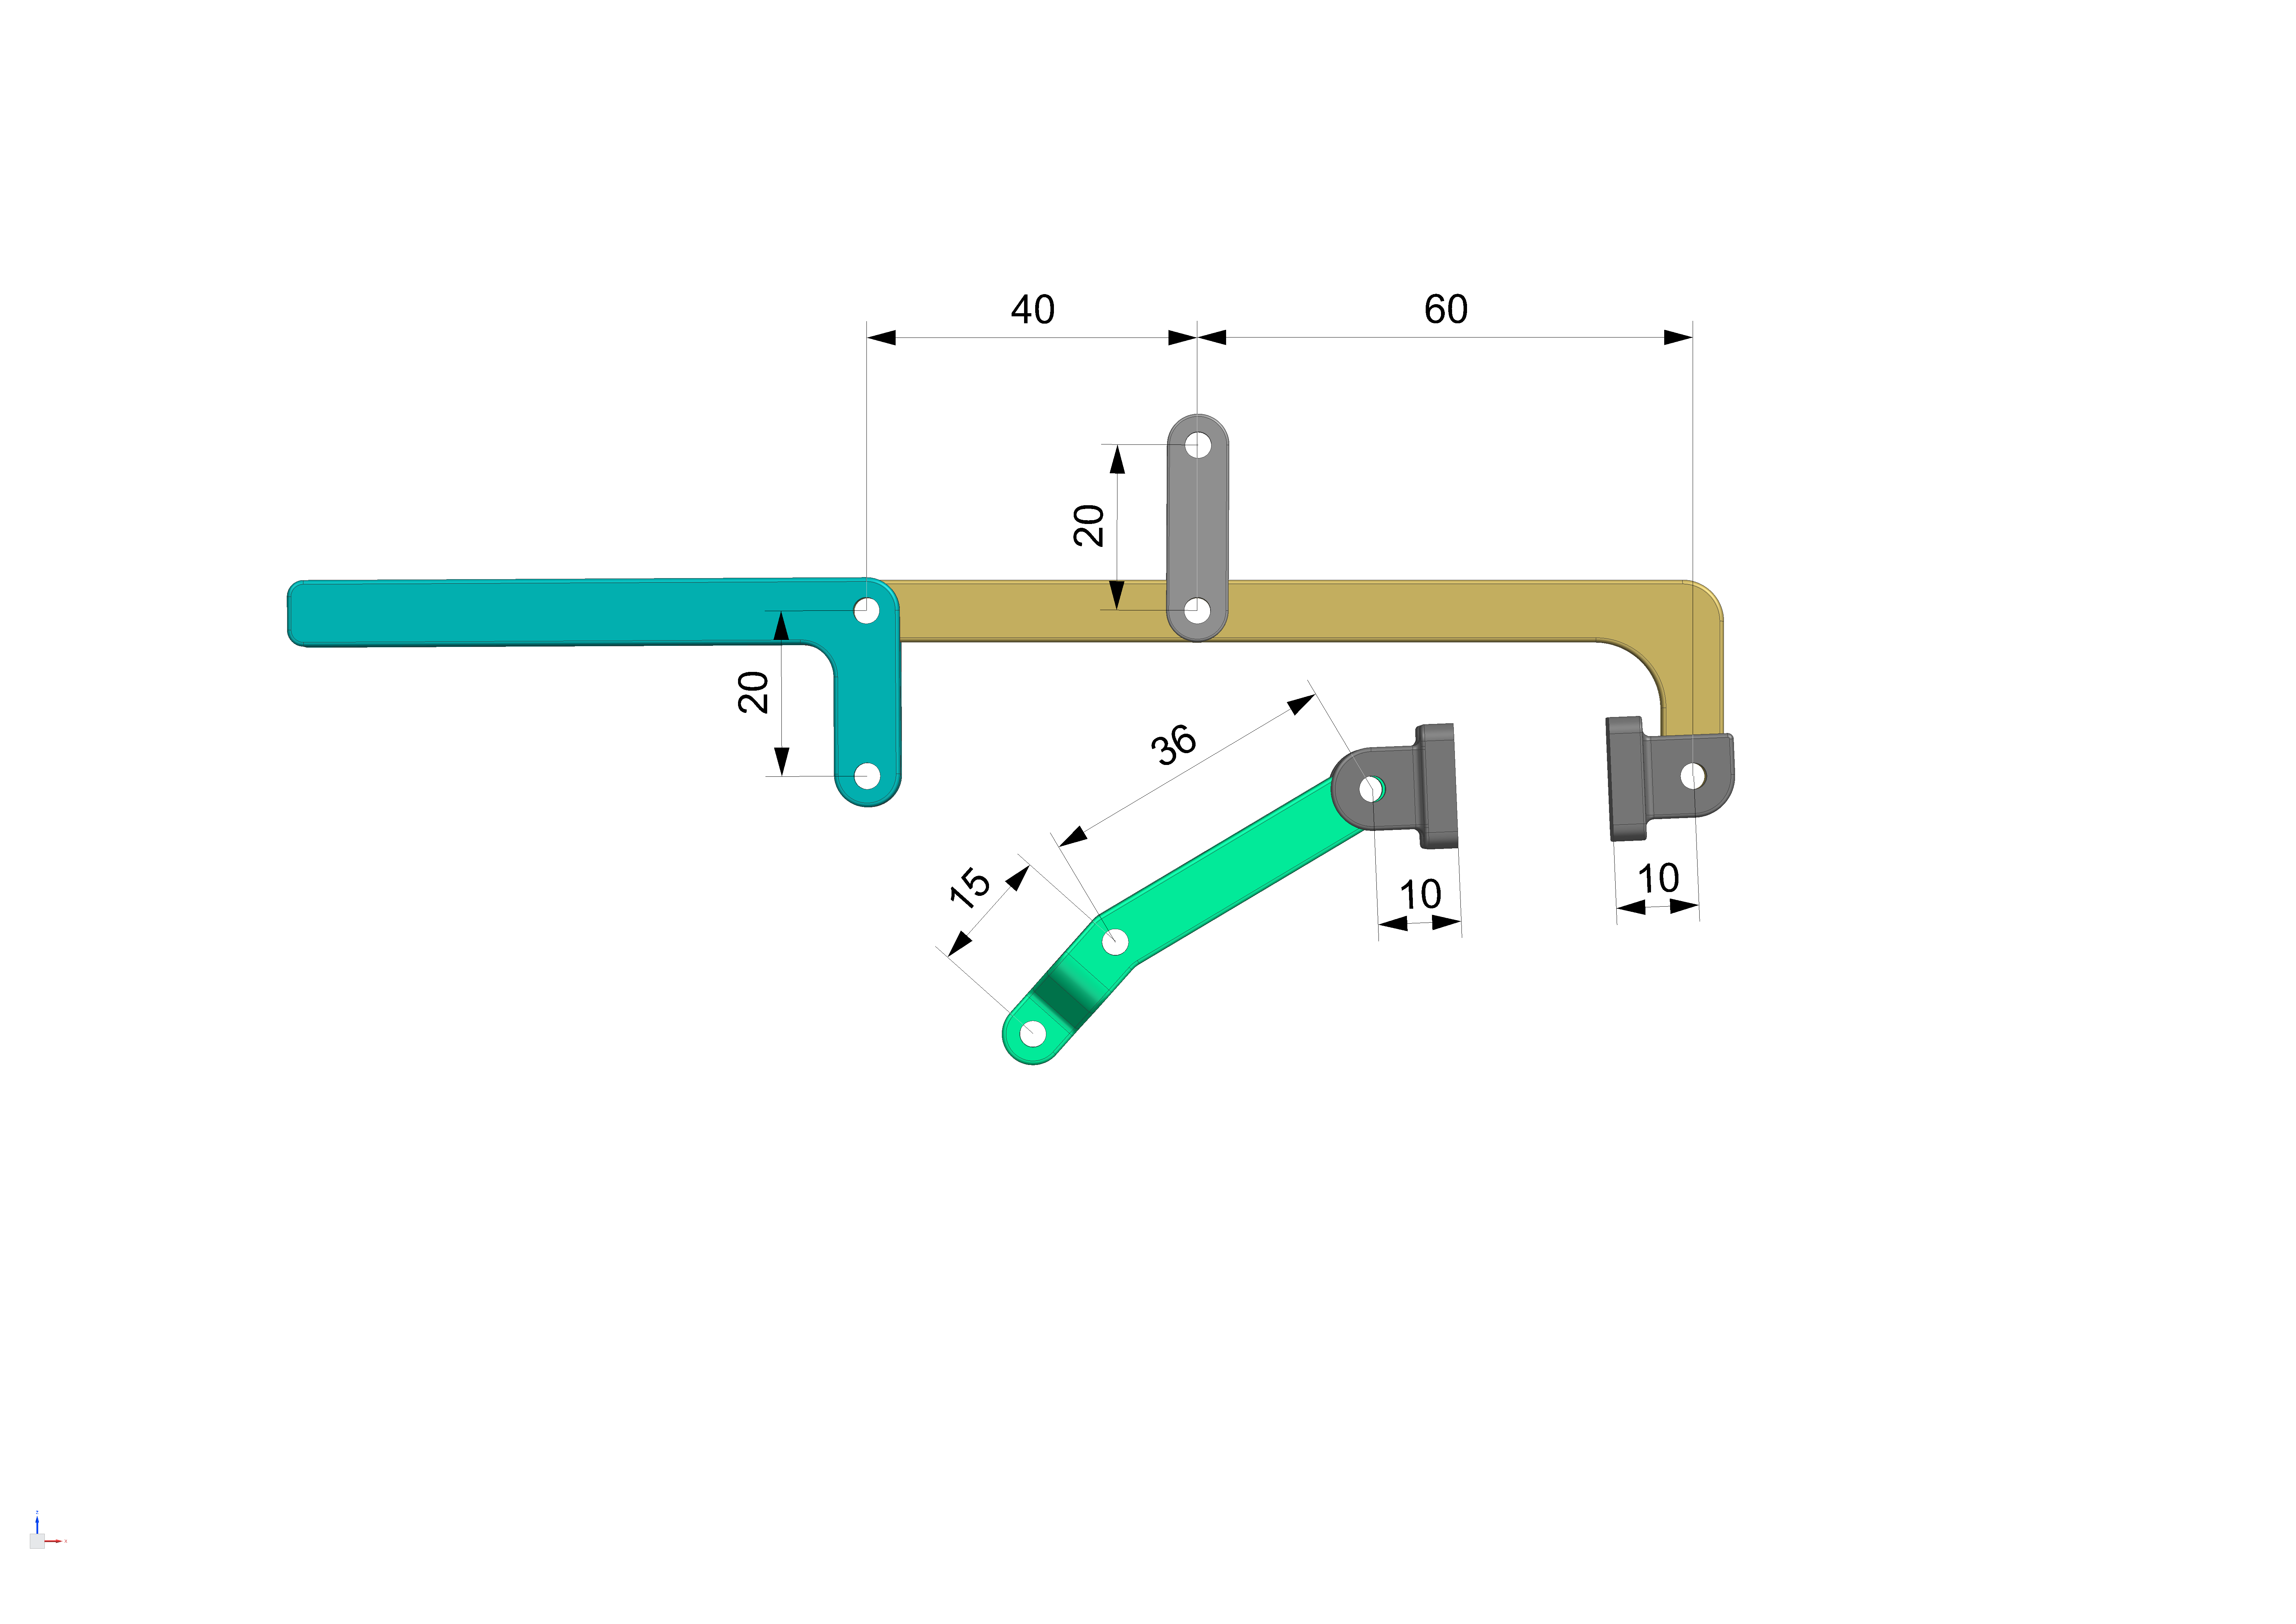
\includegraphics[width=\textwidth]{assets/greifer-prototyp/Greifer_Dimensionen_Arme.png}
\caption{Dimensionen des Gestänges}
\label{fig:gripper-linkage-dimensions}
\end{subfigure}
\caption{Dimensionen Prototyp}
\label{gripper-prototype-dimensions}
\end{figure}

Die gelenkigen Verbindungen im Prototyp wurden mit M3 Schrauben realisiert. Dies bedeutet das in den Gelenken die Gewinde der Schrauben direkt am Kunstoff der 3D-druck Teilen reiben. Eine solche Lagerung hat erhöhte Reibung und ungenaue Toleranzen zur Folge, wurde aber bewusst so gewählt da sie Kostengünstig und schnell realisiert werden kann. zur verminderung der Reibung wurden alle Gelenke mit PTFE-Trockenschmiermittel behandelt.\\
\\


\textbf{Ziele}

Mit dem Prototyp sollen folgenden Punkte getestet werden:
\begin{itemize}
    \item 1 Reibung in den Gelenken ist ausreichend gering, Gestänge lässt sich leichtgängig bewegen
    \item 2 Das Gestänge verklemmt im Betrieb nicht (keine overconstraints)
    \item 3 das Hindernis wird um mindestens 7.5mm angehoben
    \item 4 Hindernis kann zuverlässig angehoben werden (50 Testzyklen)
    \item 5 Hindernis kann auch bei bis zu 15\textdegree\ Schrägstellung angehoben werden (50 Testzyklen in verschiedenen Winkeln)
    \item 6 Hindernis wird \pm 2mm an dieselbe Stelle zurückgesetzt (50 Testzyklen)
    \item 7 Hindernis rutscht nicht aus dem Greifer bei Vibrationen (Hinderniss klemmen, Prototyp aufheben und schütteln, Hinderniss darf nicht rutschen)
    \item 8 Nötiges Drehmoment zum Anheben ist maximal gleich gross wie das ausgelegte Drehmoment (20 Ncm)
    \item 9 Die Greifbacke liegt in geöffnetem Zustand min. 5mm über dem Hindernis
\end{itemize}
\newpage

\textbf{Messungen und Beobachtungen}

\begin{table}[H]
\centering
\small
\begin{tabularx}{\textwidth}{|c|X|X|X|l|}
        \hline
        \textbf{Index} & \textbf{Kurzbeschreibung} & \textbf{Kriterium zur Erfüllung} & \textbf{Messergebnisse} & \textbf{Bemerkungen} \\
        \hline \hline
        1 & Reibung in den Gelenken & Gelenke sind leichtgängig & Das Gestänge lässt sich leicht mit einem Finger bewegen & Test erfüllt \\ \hline
        2 & Kein Verklemmen des Gestänges & Keine overconstraints festgestellt & Das Gestänge verklemmt nicht & Test erfüllt \\ \hline
        3 & Hindernis wird angehoben & Hubhöhe \geq 7.5 mm  &  9.3 \pm0.2 mm & Test erfüllt\\ \hline
        4 & Zuverlässiges Anheben & Erfolgreiche Anhebungen in 50 Zyklen & 50/50 Zyklen erfolgreich & Test erfüllt \\ \hline
        5 & Anheben bei Schrägstellung & 50 Zyklen bei bis zu 15\textdegree\ erfolgreich & 50/50 Zyklen erfolgreich & Test erfüllt \\ \hline
        6 & Rücksetzen des Hindernisses & Rücksetzgenauigkeit \pm 2 mm in 50 Zyklen& \pm1 mm in 50 Zyklen & Test erfüllt \\ \hline
        7 & Kein Rutschen bei Vibrationen & Hindernis bleibt fixiert & Hindernis verrutsch auch bei starkem Schütteln nicht & Test erfüllt \\ \hline
        8 & Max. Drehmoment  & Gemessenes Drehmoment \leq 20 Ncm & 17 Ncm & Test erfüllt \\ \hline
        9 & Greifbacke über Hindernis & Abstand \geq 5 mm im geöffneten Zustand & 12 mm & Test erfüllt \\ \hline
\end{tabularx}
    \caption{Testergebnisse der einzelnen Punkte des Prototyps.}
\label{tab:testpunkte}
\end{table}


\textbf{Fazit}

in progress...


\textbf{Weiteres Vorgehen}

in progress...


\subsubsection{Fahrwerk}

Auf Basis des Gesamtkonzepts wurde anschliessend ein Prototyp für das Fahrwerk konstruiert. Die Baugruppe Prototyp Fahrwerk beinhaltet alle für die selbständige Fortbewegung notwendigen Elemente wie Motoren, Akkus, Liniensensoren und Steuerungseinheiten.  Bei diesem Prototyp stand der einfache und zweckmässige Aufbau im Vordergrund. Bei der Grundplatte wurde darauf geachtet das verschiedene  Versionen von Systemen einfach aufgebaut und ausgetauscht werden können. Ein flexibeler Prototyp ist Ressourcenschonend. Mehr Informationen dazu gibt es im Kapitel \ref{section:Nachhaltigkeit} Nachhaltigkeit. 

In progress...
